\chapter{Implementacja}
\label{chap:implementacja}

\section{Struktura projektu}
\label{sec:struktura-projektu}
W tym podrozdziale przedstawiono logiczną i fizyczną strukturę projektu. Uwzględniono przy tym podział na projekty aplikacji klienckiej oraz API, gdyż stanowią one tak na prawdę niezależne rozwiązania (ang.~\emph{solution}) w środowisku programistycznym Visual Studio 2019.

\subsection{Struktura fizyczna projektu}
\label{sec:struktura-fizyczna-projektu}
Obie aplikacje (aplikacja kliencka i API) znajdują się w tym samym repozytorium Git. Pliki ich rozwiązań znajdują się w folderze głównym repozytorium. W folderze tym znajduję się także plik \texttt{.gitignore}. Projekty należące do rozwiązań znajdują się w folderze \texttt{src}. W katalogu \texttt{Zoltaniecki.IDP} znajduję się potrzebny do testów dostawca tożsamości, będący tylko wydmuszką prawdziwego serwisu. Strukturę głównego folderu można zobaczyć na rysunku~\ref{fig:fiz-1}.
\begin{figure}[ht]
	\centering
	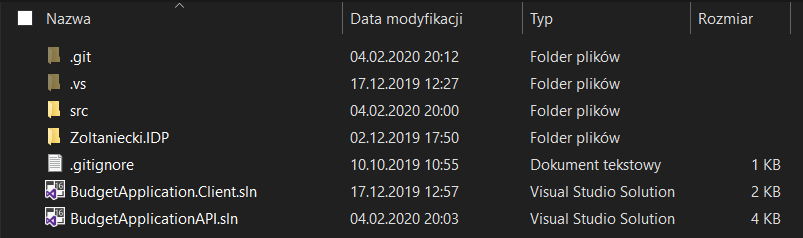
\includegraphics[scale=.77]{rys04/struktura-fizyczna-1.PNG}
	\caption{Struktura fizyczna repozytorium}
	\label{fig:fiz-1}
\end{figure}

W folderze \texttt{src} znajdują się dwa następne foldery: \texttt{API} oraz \texttt{Client}. Znajdują się w nich kolejno projekty dla rozwiązania: \texttt{BudgetApplicationAPI.sln} i~dla rozwiązania \texttt{BudgetApplicationClient.sln} (rys.~\ref{fig:fiz-2}). 
%todo czy usunać?
\begin{figure}[ht]
	\centering
	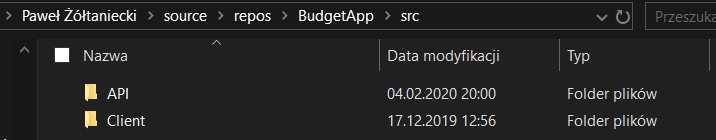
\includegraphics[scale=.77]{rys04/struktura-fizyczna-2.PNG}
	\caption{Zawartość folderu src}
	\label{fig:fiz-2}
\end{figure}

Warto zwrócić uwagę, że zarówno w API jak i w aplikacji klienckiej klasy pogrupowane są według funckjonoalności, a nie typów np.: \texttt{Services}, \texttt{Controllers}, \texttt{Views}, \texttt{Models}. Daje to dużą elastyczność i wygodę przy pracy programisty, gdyż nie musi szukać klas związanych z~jedną funkcjonalnościach w wielu w poddrzewach katalogów.

\subsubsection{Fizyczna struktura API}
Aplikacja API składa się z czterech projektów (rys.~\ref{fig:fiz-api-2}): \texttt{BudgetApplication.API}, \texttt{BudgetApplication.Domain}, \texttt{BudgetApplication.Infrastructure} oraz \texttt{BudgetApplication.QueryInfrastructure} umieszczonych w osobnych folderach. % (rys.~\ref{fig:fiz-api-1})
%%%todo czy usunać?
%%\begin{figure}[ht]
	%%\centering
	%%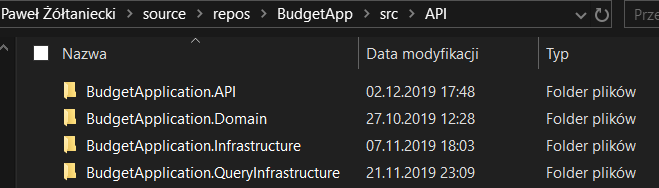
\includegraphics[scale=.77]{rys04/struktura-fizyczna-api-1.PNG}
	%%\caption{Zawartość folderu API}
	%%\label{fig:fiz-api-1}
%%\end{figure}
%Na rysunku~\ref{fig:fiz-api-2} przedstawiono strukturę rozwiązania dla API. Widać na nim cztery projekty zawierające różne foldery. 
\begin{figure}[ht]
	\centering
	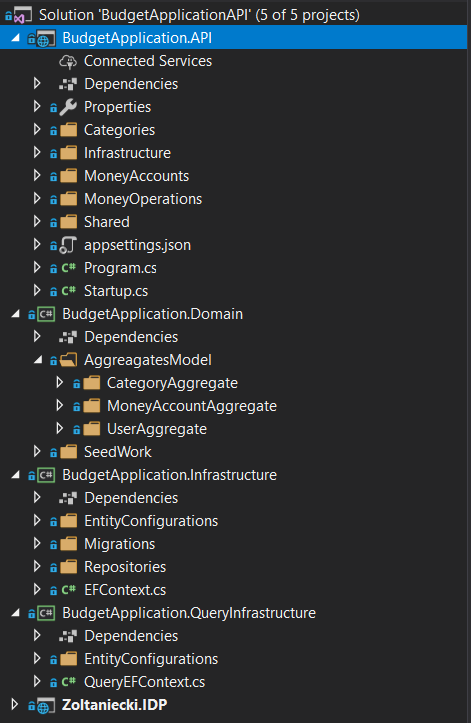
\includegraphics[scale=.77]{rys04/struktura-fizyczna-api-2.PNG}
	\caption{Struktura rozwiązania API}
	\label{fig:fiz-api-2}
\end{figure}

Foldery projektu \texttt{API} zawierają pogrupowane według funkcjonalności klasy kontrolerów API (ang.~\emph{controllers}), a także klasy związane z opisaną w sekcji~\ref{subsec:mediator} biblioteką \texttt{MediatR}: handlery (ang.~\emph{handlers}), komendy (ang.~\emph{commands}) i odpowiedzi(ang.~\emph{responses}). Katalog \texttt{Shared} zawiera współdzielone interfejsy. 

W projekcie \texttt{Domain} podkatalogi katalogu \texttt{AggregatesModel} zawierają pogrupowane według funkcjonalności encje, ich serwisy domenowe, klasy wyjątków domenowych, enumeratory, klasy typu \texttt{DTO} (ang.~\emph{Data transfer object}), a także inne klasy związane z przetwarzaniem logiki biznesowej. Folder \texttt{SeedWork} zawiera związane z taktycznym DDD interfejsy i klasy bazowe. \texttt{Program.cs} zawiera funkcję \texttt{Main}, czyli punkt wejścia do programu, a w klasie \texttt{Startup} konfigurowana jest aplikacja i jej serwisy.

Projekty \texttt{Infrastructure} i \texttt{QueryInfrastructure} zawierają warstwę dostępu do danych kolejno dla komend i zapytań, związanych z zastosowanym wzorcem \texttt{CQRS}, opisanym w punkcie~\ref{subsec:cqrs}. Foldery \texttt{EntityConfigurations} zawierają mapowania relacyjno-obiektowe charakterystyczne dla Entity Framework Core. Folder \texttt{Repositories} zawiera implementacje wzorca repozytorium dla klas encji biznesowych. Natomiast katalog \texttt{Migrations} zawiera pliki migracji modelu w bazie danych.


\subsubsection{Fizyczna struktura aplikacji klienckiej}

Aplikacja kliencka składa się z dwóch projektów (rys.~\ref{fig:fiz-client-2}): \texttt{BudgetApplication.Client} oraz \texttt{BudgetApplication.Client.Core} umieszczonych w osobnych folderach. 
%%\begin{figure}[ht]
	%%\centering
	%%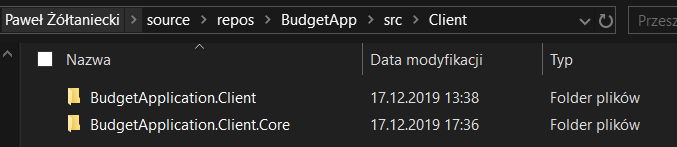
\includegraphics[scale=.77]{rys04/struktura-fizyczna-client-1.PNG}
	%%\caption{Zawartość folderu Client}
	%%\label{fig:fiz-client-1}
%%\end{figure}
%Na rysunku~\ref{fig:fiz-client-2} przedstawiono strukturę rozwiązania aplikacji klienckiej.
\begin{figure}[htb]
	\centering
	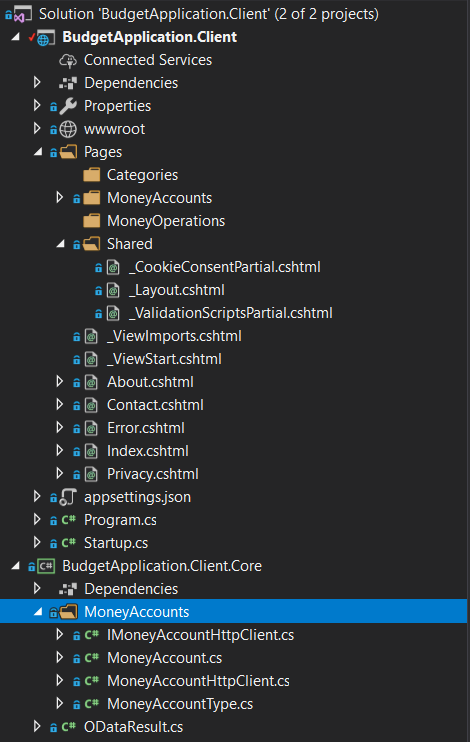
\includegraphics[scale=.77]{rys04/struktura-fizyczna-client-2.PNG}
	\caption{Struktura rozwiązania aplikacji klienckiej}
	\label{fig:fiz-client-2}
\end{figure}

Pierwszy z projektów zawiera jeden główny folder z widokami i ich modelami strony (ang.~\emph{page model}), pogrupowanymi w foldery według funkcjonalności. W głównym folderze znajdują się też widoki niezwiązane z modelami strony, a także folder \texttt{Shared} z widokami częściowymi używanymi przez pozostałe widoki. Pliki: \texttt{Program.cs} i \texttt{Startup.cs} pełnią podobną funkcję co w projekcie API.

Drugi z projektów, także zawiera tylko jeden główny katalog. Zawiera on odpowiednio skonfigurowane klasy klientów HTTP, komunikujące się z API, a także klasy modeli, które są zwracane przez zakończone sukcesem żądania HTTP.

Klasa \texttt{ODataResult} jest klasą odpowiedzi żądań HTTP GET. Zawiera ona właściwości takie jak: \emph{Count}, \emph{Metadata}, \emph{Context} i \emph{Value}, ściśle związana z implementacją protokołu OData -- punkt~\ref{subsec:odata}. Pole Value jest polem generycznym w zależności od zwracanego przez żądanie HTTP modelu. 


\subsection{Struktura logiczna projektu}
\label{sec:struktura-logiczna-projektu}
Poniżej zaprezentowano logiczną strukturę projektu. Pokazano też zależności między projektami zawartymi w rozwiązaniach dla aplikacji klienckiej oraz API.

\subsubsection{Logiczna struktura API}
Aplikacja API składa się z czterech projektów: \texttt{BudgetApplication.API}, \texttt{BudgetApplication.Domain}, \texttt{BudgetApplication.Infrastructure} oraz \texttt{BudgetApplication.QueryInfrastructure} z zależnościami jak na rysunku~\ref{fig:api-arch}. 
\begin{figure}[ht]
	\centering
	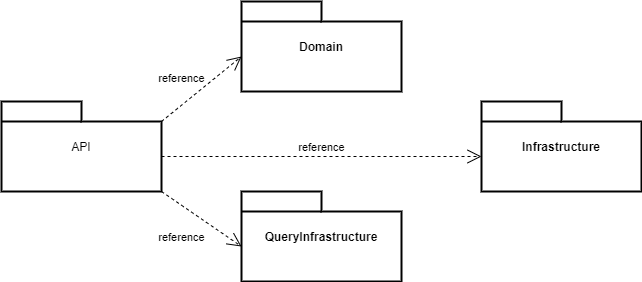
\includegraphics[scale=.55]{rys04/api-arch.png}
	\caption{Zależności między projektami w API}
	\label{fig:api-arch}
\end{figure}

Projekt \texttt{API} zawiera API kontrolery, a także handlery, odpowiedzi i żądania MediatR. Razem składają się one na warstwę aplikacji. Warstwa aplikacji operuje na obiektach domenowych, dlatego też projekt \texttt{API} zależny jest od projektu \texttt{Domain}.

Projekt \texttt{Domain} jest projektem ślepym i nie ma żadnych zależności. Znajduje się w nim kod niezależny od innych zewnętrznych frameworków. Definiuje on zachowania biznesowe obiektów domenowych, które są używane podczas wykonywania komend CQRS, wcześniej opisanych w punkcie~\ref{subsec:cqrs}. Model domenowy jest szczególnie istotny z punktu widzenia zachowania prawidłowego stanu systemu w trakcie i po wykonaniu operacji.

Warstwę persystencji dla encji domenowych stanowi projekt \texttt{Infrastructure}. Znajdują się w nim m.in. repozytoria, które implementują kontrakt zdefiniowany w projekcie \texttt{Domain}. Repozytoria korzystają z mapera relacyjno-obiektowego Entity Framework Core. Ten projekt tworzony jest dla zachowania niezależności domeny od zewnętrznych frameworków.

Projekt \texttt{QueryInfrastructure} to projekt dostarczający uproszczoną wersję modelu zapisanego w bazie danych, bez logiki domenowej. Obiekty tworzone w tej części aplikacji potrzebne są dla wykonania zapytań CQRS -- punkt~\ref{subsec:cqrs}. Projekt stworzono, podobnie jak poprzedni, również z wykorzystaniem Entity Framework Core. Oba projekty są niezależne i nic nie stoi na przeszkodzie, aby zamiast EF Core wykorzystać technologię wbudowaną w Net Framework -- ADO.NET czy bibliotekę innego mapera relacyjno-obiektowego -- \texttt{Dapper}.

\subsubsection{Logiczna struktura aplikacji klienckiej}

Aplikacja kliencka składa się z dwóch projektów: \texttt{BudgetApplication.Client} oraz \texttt{BudgetApplication.Client.Core} z zależnościami jak na rysunku~\ref{fig:client-arch}.

\begin{figure}[ht]
	\centering
	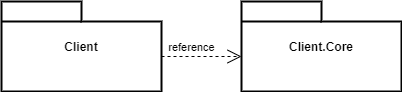
\includegraphics[scale=.55]{rys04/client-arch.png}
	\caption{Zależności między projektami w aplikacji klienckiej}
	\label{fig:client-arch}
\end{figure}

Projekt \texttt{Client} zawiera strony Razor Pages, które odpowiedzialne są za prezentowanie danych użytkownikowi i zapewnianie mu interfejsu do dokonywania zmian w systemie.

\texttt{Client.Core} zawiera klasy odpowiedzialne za komunikację z API i dostarczanie danych potrzebnych na stronach aplikacji.


\section{Szczegóły implementacji}
\label{sec:szczegoly-implementacji}
W tym podrozdziale opisano szczegóły implementacji API oraz aplikacji klienckiej. 

\subsection{Szczegóły implementacji API}
\label{subsec:szczegoly-implementacji-api}
Żądania HTTP wysłane do API przechodzą przez moduł routingu (ang.~\emph{Routing Middleware}) frameworka ASP.NET MVC. To on decyduje, do którego kontrolera i do jakiej jego akcji skierować żądanie. Jest to szczególnie istotne w bardziej skomplikowanych scenariuszach. Jednym z takich scenariuszy jest używanie implementacji protokołu OData równocześnie z routingiem atrybutowym (ang.~\emph{attribute routing}). Aby dodać routing OData do API, wystarczy w metodzie \texttt{Configure} klasy \texttt{Startup} dodać kod widoczny na listingu~\ref{list:odata-route-config}. Konfiguruje on prefix ścieżki do zasobów OData na \texttt{/api/odata}. Umożliwia on także na używanie selekcji, filtrowania, sortowania, zliczania, a także rozszerzania i stronicowania zasobu OData. 

Metoda \texttt{GetEdmModel} buduje model OData na podstawie klas encji przechowywanych w~bazie danych. Model mapowany jest do dalszej części ścieżki zasobów adresu URL za pomocą parametru przekazywanego do metody \texttt{EntitySet}. Wartość tego parametru musi być taka sama jak atrybut routingu w kontrolerze OData. Na podstawie modelu EDM generowane są metadane dla zasobów. 

{\belowcaptionskip=-10pt
\begin{lstlisting}[label=list:odata-route-config,
    caption=Konfiguracja rouingu OData w aplikacji MVC]
app.UseMvc(routeBuilder =>
{
    AddOdataRoutes(routeBuilder);
});
...
private static void AddOdataRoutes(Microsoft.AspNetCore.Routing.IRouteBuilder routeBuilder)
{
    routeBuilder.EnableDependencyInjection();
    routeBuilder.Select().Filter().OrderBy().Count().Expand().MaxTop(100).SkipToken();
    routeBuilder.MapODataServiceRoute("odata", "api/odata", OdataExtensionsMethods.GetEdmModel());
}
...
internal static IEdmModel GetEdmModel()
{
    var builder = new ODataConventionModelBuilder();

    builder.EntitySet<Category>("categories");
    builder.EntitySet<MoneyAccount>("money-accounts");
    builder.EntitySet<MoneyOperation>("money-operations");
    builder.EntitySet<Expense>("expenses");
    builder.EntitySet<Income>("incomes");

    return builder.GetEdmModel();
}
\end{lstlisting}
}

Kontroler OData i standardowy kontroler API różnią się od siebie pod kilkoma względami. Standardowy kontroler API dziedziczy po klasie \texttt{ControllerBase} i używa atrybutów routingu \texttt{Route} z przestrzeni nazw \texttt{Microsoft.AspNetCore.Mvc}. Natomiast kontroler OData dziedziczy po klasie \texttt{ODataController}. Dzięki zastosowaniu klasy \texttt{ODataController} kontroler OData m.in.~zwraca dane w~formacie zgodnym z protokołem OData, czyli opakowuje dane w~pole \texttt{values}, zapewnia link do metadanych zasobu, a także odpowiednie nagłówki charakterystyczne dla protokołu. Kontroler OData używa także innych atrybutów routingu: \texttt{ODataRoute} dla pojedynczej akcji oraz \texttt{ODataRoutePrefix} dla określenia prefixu routingu dla wszystkich akcji kontrolera. Znajdują się one w przestrzeni nazw \texttt{Microsoft.AspNet.OData.Routing}. Zastosowanie nieodpowiednich atrybutów routingu skutkuje błędem dopasowania wielu akcji do jednego adresu (ang.~\emph{AmbiguousActionException: Multiple actions matched}) lub zwróceniem statusu HTTP 404. Na listingu~\ref{list:api-ctrl-1} oraz~\ref{list:odata-ctrl-1} przedstawiono przykłady implementacji obu kontrolerów. Część kodu została pominięta dla klarowności.

Ponadto w kontrolerze OData używane są atrybuty \texttt{EnableQuery}. Zezwalają one na korzystanie w adresie URL z opcji filtrowania, sortowania itd., skonfigurowanych w metodzie \texttt{AddOdataRoutes} na listingu~\ref{list:odata-route-config}. Brak tych atrybutów dla konkretnej akcji skutkować będzie brakiem obsługi tych funkcjonalności. Ścieżka wyszukiwania (ang.~\emph{query string} będzie w tym wypadku ignorowana. Istnieje też atrybut \texttt{Queryable}, który można wykorzystać do ograniczenia funkcjonalności, które programista chce udostępnić w akcji. Robi się to za pomocą przekazania do atrybutu podzbioru skonfigurowanych opcji wyszukiwania OData. Tutaj przykład atrybutu ograniczającego opcje wyszukiwania do stronicowania: \texttt{[Queryable(AllowedQueryOptions=
    AllowedQueryOptions.Skip | AllowedQueryOptions.Top)]}

{\belowcaptionskip=-10pt
\begin{lstlisting}[label=list:api-ctrl-1,
    caption=Przykład implementacji standardowego kontrolera API]
[Route("api/money-accounts")]
[ApiController]
public class MoneyAccountsController : ControllerBase
{
    private readonly IMediator _mediator;
...
    //Patch api/money-accounts/1
    [HttpPatch]
    [Route("{moneyAccountId}")]
    public async Task<IActionResult> UpdateAccount(Guid moneyAccountId,
        UpdateMoneyAccountCommand updateMoneyAccountCommand)
    {
        updateMoneyAccountCommand.MoneyAccountId = moneyAccountId;
        bool result = await _mediator.Send(updateMoneyAccountCommand);
    
        if (!result)
        {
            return BadRequest();
        }
    
        return Ok();
    }
}
\end{lstlisting}
}

{\belowcaptionskip=-10pt
\begin{lstlisting}[label=list:odata-ctrl-1,
    caption=Przykład implementacji kontrolera OData]
[ODataRoutePrefix("money-accounts")]
public class ODataMoneyAccountController : ODataController
{
    private readonly QueryEFContext _moneyAccountRepository;
...
    [EnableQuery]
    [ODataRoute("{id}")]
    public ActionResult<MoneyAccount> GetAsync(Guid id)
    {
        return Ok(_moneyAccountRepository.MoneyAccounts
            .Where(acc => acc.Id == id));
    }
}
\end{lstlisting}
}

W systemie aplikacji domowego budżetu kontrolery OData są używane tylko do żądań HTTP GET, a kontrolery API do wszystkich innych żądań, które zmieniają stan systemu.
Kontroler OData bezpośrednio korzysta z kontekstu do bazy danych, który zwraca kolekcję implementują generyczny interfejs \texttt{IQueryable}. Dzięki temu OData jest w stanie przenieść logikę zapytania do bazy danych.

Standardowy kontroler API korzysta z mediatora, aby wysłać komendę do kolejnej warstwy aplikacji, w której zachodzą procesy biznesowe. Przykład serwisu aplikacji, który przetwarza komendę pokazano na listingu~\ref{list:handler-impl}. Operuje on na encjach i serwisach domenowych. W tym wypadku wykorzystano repozytorium do pobrania konta bankowego z bazy danych. Następnie do konta bankowego dodawany jest nowy wydatek, a całość zapisywana jest z zastosowaniem wzorca \texttt{Unit of Work}, który gwarantuje, że zmiany, które zaszły w systemie będą zapisane w~jednej transakcji bazodanowej. 

{\belowcaptionskip=-10pt
\begin{lstlisting}[label=list:handler-impl,
    caption=Przykład implementacji handlera aplikacji]
public async Task<CreateExpenseResponse> Handle(CreateExpenseCommand command, CancellationToken cancellationToken)
{
    var accountId = command.AccountId;
    var expenseDTO = _mapper.Map<AddExpenseDTO>(command);
    MoneyAccount moneyAccount = await _moneyAccountRepository.GetAsync(accountId);

    IReadOnlyExpense operation = moneyAccount.AddOperation(expenseDTO);

    _moneyAccountRepository.Update(moneyAccount);
    bool success = await _moneyAccountRepository.UnitOfWork.SaveEntitiesAsync();

    return success ? _mapper.Map<CreateExpenseResponse>(operation) : null;
}
\end{lstlisting}
}

\subsection{Szczegóły implementacji aplikacji klienckiej}
\label{subsec:szczegoly-implementacji-client}

Żądania użytkownika wysyłane do aplikacji klienckiej mapowane są do konkretnych stron Razor Pages. Strona Razor Page składa się z widoku napisanego przy pomocą języka html i opcjonalnie modelu strony (ang.~\emph{page model}). Na stronie często też znajdują się dodatkowe komendy składni Razor, których zadaniem jest budowanie widoku w zależności od modelu przekazanego do strony, a także generowanie widoków częściowych (ang.~\emph{partial views}). Widoki częściowe ułatwiają wydzielanie wspólnych części widoku strony do oddzielnych plików. Można łatwo wykorzystać je w różnych stronach Razor, a także użyć w pętli dla kolekcji obiektów zawartych w modelu widoku. Widoki częściowe nie mogą mieć swoich modeli strony, a jedynie polegają na danych przekazanych do nich z zewnątrz.

Aby widok był stroną Razor Page musi na nim znaleźć się dyrektywa \texttt{@page}. Służy ona także do routingu w aplikacji. Domyślnie routing oparty jest o strukturę folderów i nazwę strony. Oczywiście w takiej formie jest niewystarczający. Na listingu~\ref{list:razor-page-1} pokazano przykład wykorzystania dyrektywy \texttt{@page} do stworzenia strony konta bankowego o konkretnym identyfikatorze typu \texttt{guid} -- linia 1.

{\belowcaptionskip=-10pt
\begin{lstlisting}[label=list:razor-page-1,
    caption=Przykład strony Razor Page: \texttt{Edit.cshtml}]
@page "{accountId:guid?}"
@model BudgetApplication.Client.Pages.MoneyAccounts.EditModel
...
<h2>Edycja konta: @Model.MoneyAccount.Name</h2>
@if (Model.Message != null)
{
    <div class="alert alert-info">@Model.Message</div>
}
<form method="post">
  <input type="hidden" asp-for="MoneyAccount.Id" />

  <div class="form-group">
    <label asp-for="MoneyAccount.Name"></label>
    <input asp-for="MoneyAccount.Name" class="form-control" />
    <span asp-validation-for="MoneyAccount.Name" class="text-danger"></span>
  </div>
  ...
  <div class="form-group">
    <label asp-for="MoneyAccount.Type"></label>
    <select asp-for="MoneyAccount.Type" asp-items="Model.MoneyAccountTypes" class="form-control"></select>
    <span asp-validation-for="MoneyAccount.Type" class="text-danger"></span>
  </div>
  ...
</form>
@section Scripts {
    <partial name="_ValidationScriptsPartial" />
}
\end{lstlisting}
}

Na listingu~\ref{list:razor-page-1} pokazano także, w jaki sposób za pomocą składni Razor napełnić widok danymi z modelu strony. Przykładem takiej dyrektywy jest ta w linijce 4. Dyrektywy używające modelu strony mogą posłużyć także do warunkowego generowania części widoku -- linie 5-7.

Strona z listingu~\ref{list:razor-page-1} zawiera dyrektywę Razor \texttt{@model}. Określa ona typ modelu strony przypisanego do strony. Jego nazwa składa się z nazwy strony i doklejonego do niej przyrostka \texttt{Model}. Model strony jest ściśle powiązany ze stroną. Jest tzw. klasą ,,code-behind''. Pomiędzy widokiem strony Razor i modelem strony jest wiązanie, które sprawia, że zmiany na widoku odzwierciedlane są w modelu, a zmiany w modelu odzwierciedlane są na stronie. Ten proces ma miejsca poprzez synchroniczne żądania HTTP, w trakcie działań użytkownika, takich jak: wejście na stronę, odświeżenie strony, naciśnięcie guzika. Jest to realizacja popularnego wzorca architektonicznego \texttt{MVVM} (ang.~\emph{Model–view–viewmodel}).

Model strony to klasa dziedzicząca po klasie \texttt{PageModel}. Implementuje on dwie metody: \texttt{OnGetAsync} oraz \texttt{OnGetAsync}. W pierwszej z nich implementowana jest logika pobierania danych i napełniania nimi widoku strony. Druga z nich służy do obsługi żądań HTTP POST użytkownika, a w szczególności do wysyłania formularzy. 

Na listingu~\ref{list:razor-page-model-1} przedstawiono przykład modelu strony. Zawiera on właściwość typu \texttt{MoneyAccount}. Pola jej klasy są bezpośrednio mapowane na wartości za pomocą dyrektyw Razor w pliku strony -- listing~\ref{list:razor-page-1}. W metodzie \texttt{OnGetAsync} przypisywany jest obiekt konta bankowego do tej właściwości. Warto zwrócić uwagę, że zarówno parametr metody \texttt{OnGetAsync}, jak i parametr dyrektywy routingu \texttt{@page} (listing~\ref{list:razor-page-1} linia 1) mają typ mogący być wartością \texttt{null}. Dzięki temu strona obsługuje dwie ścieżki routingu: \texttt{/Edit/{id}} do strony edycji istniejącej konta bankowego o podanym id oraz \texttt{/Edit} do strony tworzenia nowego konta bankowego. Podobna sytuacja ma miejsce w metodzie \texttt{OnPostASync}.

Atrybut \texttt{[BindProperty]} dla właściwości \texttt{MoneyAccount} sprawia, że konto bankowe tworzone jest na podstawie danych z żądania i od razu przypisywane do właściwości, dlatego metoda \texttt{OnPostAsync} nie musi mieć parametru typu \texttt{MoneyAccount}. Domyślnie ten atrybut działa tylko dla żądania POST, jednak łatwo go skonfigurować dla żądań GET. W tym przykładzie jest to niepotrzebne.

Za pomocą metody \texttt{GetEnumSelectList} tzw.\ ,,Tag Helper'', łatwo zmapowowano wartości enumeratora \texttt{MoneyAccountType} na kolekcję, wykorzystywaną w rozwijanym menu w formularzu na listingu~\ref{list:razor-page-1} - linia 18-21.

{\belowcaptionskip=-10pt
\begin{lstlisting}[label=list:razor-page-model-1,
    caption=Przykład modelu strony Razor Page: \texttt{EditPage.cs}]
public class EditModel : PageModel
{
...
  [BindProperty]
  public MoneyAccount MoneyAccount { get; set; }
  public IEnumerable<SelectListItem> MoneyAccountTypes { get; set; }
  public async Task<IActionResult> OnGetAsync(Guid? accountId)
  {
    MoneyAccountTypes = _htmlHelper.GetEnumSelectList<MoneyAccountType>();
    if (accountId.HasValue)
      MoneyAccount = await _accountHttpClient.GetMoneyAccountByIdAsync(accountId.Value);
    else
      MoneyAccount = new MoneyAccount();
    
    return MoneyAccount == null 
      ? RedirectToPage("./NotFound")
      : Page() as IActionResult;
  }

  public async Task<IActionResult> OnPostAsync()
  {
    if (!ModelState.IsValid)
    {
      MoneyAccountTypes = _htmlHelper.GetEnumSelectList<MoneyAccountType>();
      return Page();
    }
    try
    {
      MoneyAccount = MoneyAccount.Id == Guid.Empty 
        ? await _accountHttpClient.AddMoneyAccountsAsync(MoneyAccount)
        : await _accountHttpClient.EditMoneyAccountsAsync(MoneyAccount);

      return RedirectToPage("./Edit", new { accountId = MoneyAccount.Id });
    }
    ...
  }
}
\end{lstlisting}
}

Na końcu listingu~\ref{list:razor-page-1} znajduje się dyrektywa generująca widok częściowy w sekcji \texttt{Scripts} głównego układu strony -- plik \texttt{\_Layout.cshtml}. Odpowiada ona za generowanie na stronie \texttt{Edit.cshtml} skryptów biblioteki \texttt{jQuery unobtrusive validation}, która współpracuje z frameworkiem ASP.NET Core i zapewnia walidację po stronie klienta na podstawie adnotacji modelu klasy języka C\#. 

Przykład walidowanej klasy znajduje się na listingu~\ref{list:razor-validation-1}. Przed tagiem \texttt{body} HTML w~pliku \texttt{\_Layout.cshtml} znajduje się dyrektywa \texttt{@RenderSection("Scripts", required: false)}. Umożliwia dołączenie opcjonalnej sekcji skryptów przez widoki, korzystające z tego układu strony.


{\belowcaptionskip=-10pt
\begin{lstlisting}[label=list:razor-validation-1,
    caption=Przykład klasy z adnotacjami]
using System.ComponentModel.DataAnnotations;
public class MoneyAccount
{
    public Guid Id { get; set; }
    [Required]
    public Guid UserId { get; set; }
    [Required, MinLength(8)]
    public string Name { get; set; }
    [Required]
    public MoneyAccountType Type { get; set; }
    [MaxLength(255)]
    public string Description { get; set; }
...
    [MinLength(26)]
    [MaxLength(26)]
    public string BankAccountNumber { get; set; }
}
\end{lstlisting}
}
